\documentclass[a4paper,12pt]{article}

\usepackage[a4paper, total={6in, 9.5in}]{geometry}
\usepackage[utf8]{inputenc}
\usepackage[T1]{fontenc}
\usepackage[british]{babel}

\usepackage{graphicx}
\graphicspath{{images/}}

\usepackage{booktabs}
\usepackage{longtable}
\usepackage{lscape}

\usepackage{xcolor}
\usepackage{listings}
\lstset{basicstyle=\ttfamily,
  showstringspaces=false,
  commentstyle=\color{red},
  keywordstyle=\color{blue}
}

\newcommand\tab[1][1cm]{\hspace*{#1}}

\usepackage{mathtools}
\usepackage{amssymb}
\usepackage{enumitem}
\usepackage{lastpage}

\usepackage{fancyhdr}
\pagestyle{fancy}
\lhead{Sistemas Basados en el conocimiento}
\rhead{Page \thepage\ of \pageref{LastPage}}
\cfoot{\scriptsize{\today{}}}

\begin{document}

% First page %%%%%%%%%%%%%%%%%%%%%%%%%%%%%%%%%%%%%%%%%%%%%%%%%%%%%%%%%%%%%%
\begin{titlepage}
\begin{center}


\includegraphics[width=0.6\textwidth]{logoesi}\\[5cm]

% Title
\rule{\linewidth}{0.5mm} \\[0.4cm]
{ \huge \bfseries Sistemas Basados en el Conocimiento\\[0.4cm] }
\rule{\linewidth}{0.5mm} \\[1.5cm]
{\huge Diagnóstico de problemas mecánicos (2017/2018)}\\[0.5cm]

% Author
\large{Juan Jos\'e Corroto Mart\'in}

\end{center}
\end{titlepage}

\tableofcontents
\newpage

\section{Diccionario de conceptos}
\subsection{Glosario y Ontología}
A continuación se detalla el glosario con la definición de todos los conceptos y elementos físicos del dominio que nos ocupa:

\begin{itemize}
\item[1] \textbf{Orden de reparación}: Documento que se abre para cada nuevo cliente incluyendo datos como nombre, apellidos, teléfono, datos del vehículo y otros datos relevantes, así como datos de la empresa e y numeraciones para su control interno. Este documento es el que, de forma legal, autoriza al taller a realizar la revisión y reparación del vehículo una vez firmado por el cliente.
\item[2] \textbf{Máquina de diagnosis}: Consiste básicamente en un portátil con un software capaz de realizar numerosas cosas. Permite, entre otras cosas, diagnosticar el coche conectándolo a la centralita. Así recibiremos un código de diagnosis orientativo, que nos dirá a grandes rasgos en que parte del coche está el fallo. También ayuda medir voltajes en sistemas eléctricos del coche, y a medir presiones en sistemas mecánicos (en este caso sólo nos indica el valor objetivo que debería haber en esa parte). Además también puede forzar el accionamiento de ciertas partes eléctricas del coche, como válvulas, para comprobar que se activan correctamente.
\item[3] \textbf{código de avería}: Código que nos devuelve la máquina de diagnosis para indicar qué sistema es el que falla. Estos códigos están sujetos a estándares y por tanto son genéricos. Los códigos del estándar ISO tienen varios formatos, como los códigos P0xxx, P2xxx, B0xxx, U0xxx, entre otros. Además cualquier fabricante puede definir sus propios códigos, aunque estos definen los mismos problemas y se pueden "traducir" a códigos del estándar ISO.
\item[4] \textbf{Sensor}: Componente eléctrico que es capaz de medir una magnitud física de su entorno. Pueden medir intensidad lumínica, temperatura, distancia, aceleración, inclinación, presión, desplazamiento, fuerza, torsión, humedad, movimiento, pH, etc. Los sensores recogen esta información y la transforman en señales eléctricas. La mayoría de sensores usados en sistemas dentro de un vehículo se usan para medir presiones en zonas donde debería haber altas presiones.
\item[5] \textbf{Captador}: dispositivo que es capaz de traducir las señales que el sensor manda y convertirlas en señales entendibles por el sistema que use el captador, en nuestro caso la máquina de diagnosis. En el dominio que nos encontramos las palabras sensor y captador se suelen usar indistintamente para designar captador, porque un sensor no sirve de nada sin un captador que nos lo traduzca.
\item[6] \textbf{Turbo o turbocompresor}: es un sistema de sobrealimentación que usa una turbina centrífuga para comprimir gases. Estos gases son los que se pasan al motor de explosión del coche, logrando que haya mayor cantidad de oxígeno en la mezcla de gas con combustible. En nuestro sistema utilízaremos la palabra turbo para designar a la parte física del turbo, es decir, a la propia turbina.
\item[7] \textbf{Sistema de álabes}: sistema utilizado en los turbos de geometría variable. Éste sistema de álabes, que se pueden abrir y cerrar, permite que los gases de escape influyan con más fuerza en las paletas de la turbina, logrando así la máxima compresión del aire.
\item[8] \textbf{Electroválvula}: válvula que actúa con un electroiman y que regula el caudal de un fluido.
\item[9] \textbf{Tubo de vacío}: es tubo por el que se transportan gases sin presión.
\item[10] \textbf{MITYVAC}: colección de herramientas usadas para medir y comprobar la presión de distintas zonas en vehículos. No sólo nos permiten medir la presión de alguna parte, también nos ayuda a abrir y cerrar álabes en un turbo, para medir la presión dependiendo de si están abiertos y cerrados.
\item[11] \textbf{Válvula E.G.R}: se trata de una electroválvula que forma parte del circuito de sobrealimentación de gases en el vehículo, y se encarga de reintroducir parte de los gases que salen por el tubo de escape al sistema de admisión. 
\item[12] \textbf{Circuito de sobrealimentación de gases}: Sistema del vehículo que se encarga de circular gases hacia el motor y fuera de él hacia el tubo de escape. El turbo y la válvula E.G.R forman parte este sistema, además de todos los componentes eléctricos y manguitos y tubos de vacío que se usan para circular los gases entre las diferentes partes del vehículo.
\item[13] \textbf{Manguito}: todo elemento mecánico de conexión entre dos elementos.
\item[14] \textbf{Pistón del motor}: un motor de explosión de cuatro tiempos en un vehículo suele estar formado por cuatro pistones, elementos que suben y bajan y que se encargan de comprimir la mezcla entre aire y combustible dentro del cilindro.
\item[15] \textbf{Tubo de admisión}: tubo por el que entran los gases al turbo.
\item[16] \textbf{Eje de turbo}: Eje en torno al cuál gira la turbina del turbocompresor. Una parte de eje está en contacto con los gases de escape, que al salir calientes ya cierta presión hacen girar a la turbina, que se encarga de comprimir los gases de entrada.
\item[17] \textbf{Sensor de revoluciones}: sensor situado cerca del cig\"ue\~nal. Este sensor se encarga de comunicar las revoluciones de giro del motor y de la posición del cig\"ue\~nal y de los cilindros.
\item[18] \textbf{Sistema common-rail}: en español conducto común. Es un sistema que comprime el combustible para después ser inyectado al motor. El sistema common-rail es de diseño modular. Cada sistema cuenta con una bomba de alta presión, varios inyectores, un raíl y una unidad de control electrónica. A diferencia de los sistemas de inyección convencionales, en los que la generación de presión y la inyección se realizan a la vez, en el sistema common-rail se realizan por separado, y el combustible viaja por un carril común a los diferentes inyectores.
\end{itemize}

También podemos ver una red semántica con los conceptos anteriores y las relaciones entre ellos:\\\\
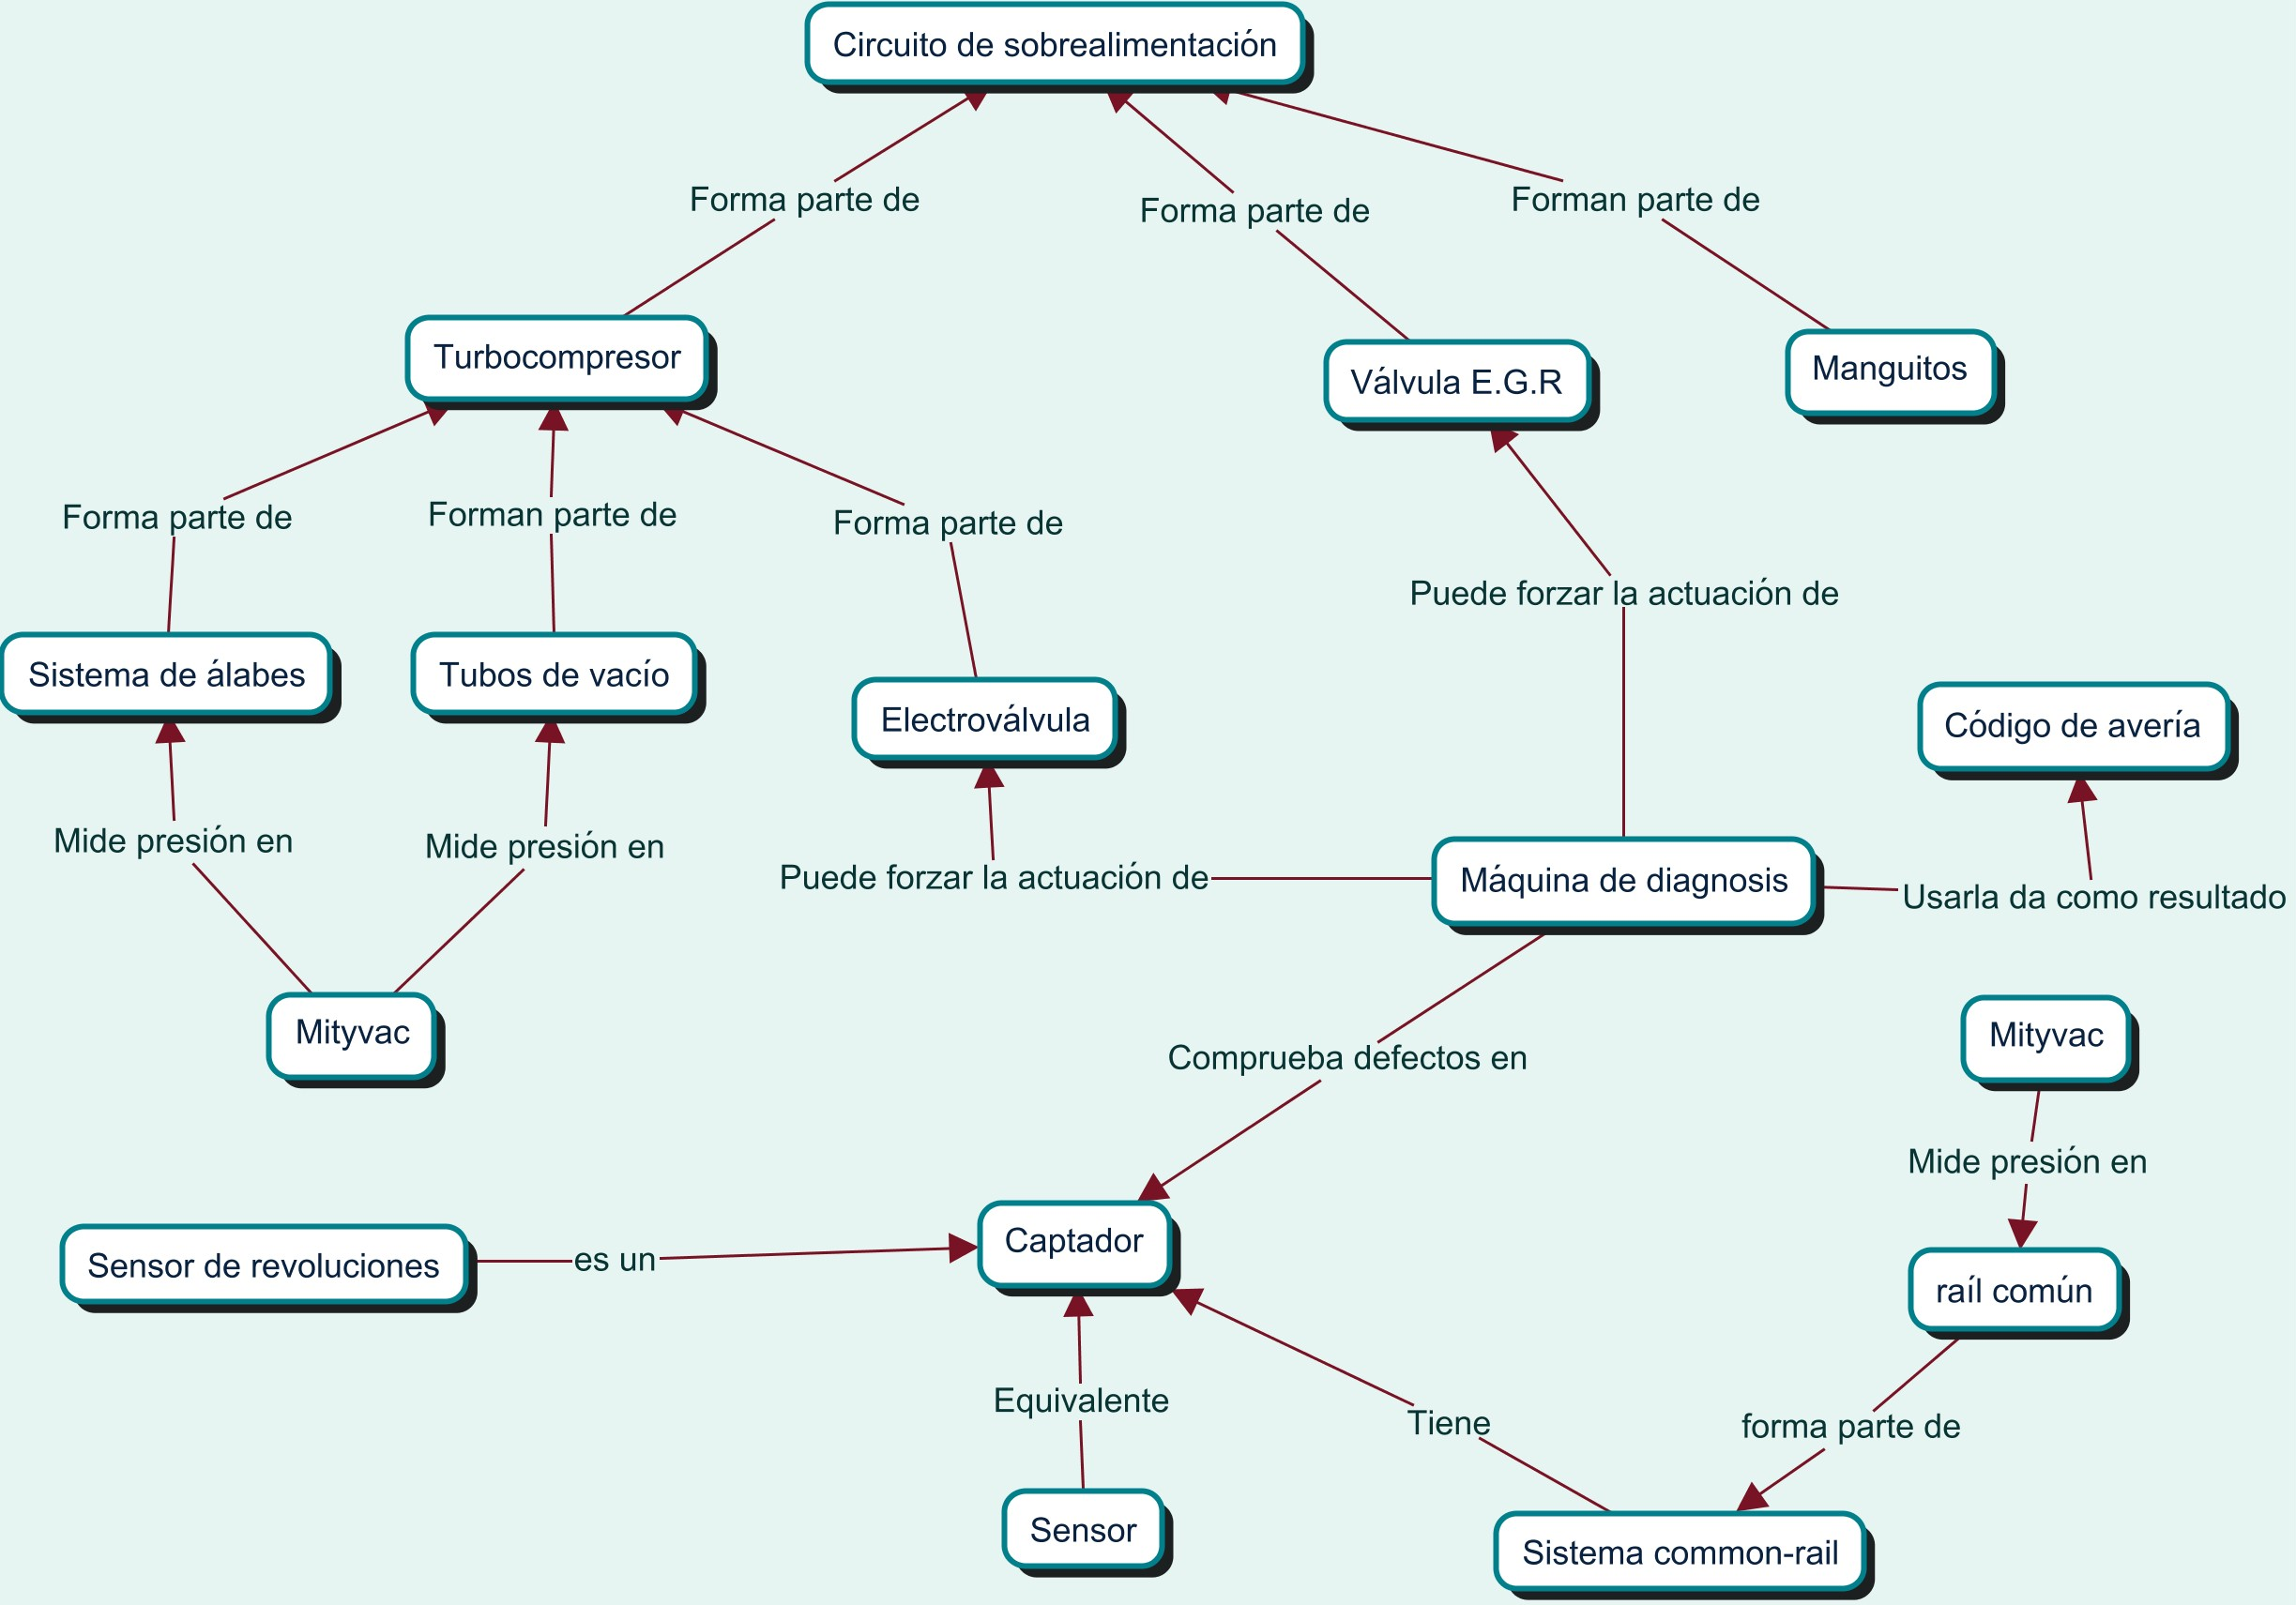
\includegraphics[scale=0.175]{red.jpg}

\newpage
\subsection{Tabla Objeto-Atributo-Valor}
A continuación se muestra la tabla Objeto-Atributo-Valor con los objetos que se van a modelar en el sistema junto con sus valores.

\begin{table}[h]
\centering
\caption{Tabla Objeto-Atributo-Valor}
\label{my-label}
\begin{tabular}{@{}lll@{}}
\toprule
Objeto                                                                                        & Atributo                                                                                        & Valor                                            \\ \midrule
\multicolumn{1}{|l|}{\begin{tabular}[c]{@{}l@{}}Sistema de \\ Sobrealimentación\end{tabular}} & \multicolumn{1}{l|}{Manguitos}                                                                  & \multicolumn{1}{l|}{\{Buen estado, Mal estado\}} \\ \cmidrule(l){2-3} 
\multicolumn{1}{|l|}{}                                                                        & \multicolumn{1}{l|}{Presión}                                                                    & \multicolumn{1}{l|}{\{Correcta, Deficiente\}}    \\ \cmidrule(l){2-3} 
\multicolumn{1}{|l|}{}                                                                        & \multicolumn{1}{l|}{\begin{tabular}[c]{@{}l@{}}Funcionamiento de\\ Válvula E.G.R\end{tabular}}  & \multicolumn{1}{l|}{\{Correcta, Deficiente\}}    \\ \midrule
\multicolumn{1}{|l|}{Turbocompresor}                                                          & \multicolumn{1}{l|}{\begin{tabular}[c]{@{}l@{}}Presión en\\ Tubos de vacío\end{tabular}}        & \multicolumn{1}{l|}{\{Correcta, Deficiente\}}    \\ \cmidrule(l){2-3} 
\multicolumn{1}{|l|}{}                                                                        & \multicolumn{1}{l|}{\begin{tabular}[c]{@{}l@{}}Funcionamiento de\\ Electroválvula\end{tabular}} & \multicolumn{1}{l|}{\{Correcta, Deficiente\}}    \\ \cmidrule(l){2-3} 
\multicolumn{1}{|l|}{}                                                                        & \multicolumn{1}{l|}{Presión en álabes}                                                          & \multicolumn{1}{l|}{\{Correcta, Deficiente\}}    \\ \cmidrule(l){2-3} 
\multicolumn{1}{|l|}{}                                                                        & \multicolumn{1}{l|}{Holgura del eje}                                                            & \multicolumn{1}{l|}{\{Correcta, Deficiente\}}    \\ \midrule
\multicolumn{1}{|l|}{Sensor de revoluciones}                                                  & \multicolumn{1}{l|}{Sistema Eléctrico}                                                          & \multicolumn{1}{l|}{\{Correcta, Deficiente\}}    \\ \midrule
\multicolumn{1}{|l|}{Common-rail}                                                             & \multicolumn{1}{l|}{Sistema Eléctrico}                                                          & \multicolumn{1}{l|}{\{Correcta, Deficiente\}}    \\ \cmidrule(l){2-3} 
                                                                                              & \begin{tabular}[c]{@{}l@{}}Presión en el carril\\ común\end{tabular}                            & \{Correcta,Deficiente\}                          \\ \bottomrule
\end{tabular}
\end{table}

\section{Metaconocimiento}
A parte del metaconocimiento que se puede extraer de la ontología presentada anteriormente, también se dispone de cierto metaconocimiento más abstracto. Este conocimiento ha sido extraído de la experiencia y conocimiento heurístico del experto:

\begin{itemize}
\item Si se observan los síntomas pérdida de presión y humo blanco, además del código de avería en el circuito de sobrealimentación de gases, se puede pasar directamente a ver si el turbo tiene el problema, en vez de mirar primero el sistema de sobrealimentación, tubos de vacío, etc.
\end{itemize}
\begin{landscape}
\section{Mapa de conocimientos}
\includegraphics[scale=0.155]{mapa.jpg}
\end{landscape} 
\newpage
\section{Representación del conocimiento}
En esta sección se presentarán las reglas que van a mover nuestro sistema:

\begin{itemize}
%\item[1.]\textbf{Si}\\ \tab cosa\\ \tab y cosa 2\\ \tab y cosa 3\\ \textbf{Entonces}\\ \tab Conclusión 1\\ \tab Conclusión 2
\item[1.]\textbf{Si}\\ \tab No hay código de error\\\textbf{Entonces}\\ \tab Obtener código de error
\item[2.]\textbf{Si}\\ \tab pérdida de potencia\\ \tab y echa humo blanco\\ \tab y P0400\\ \textbf{Entonces}\\ \tab Mirar eje del turbo\\ \tab \textbf{Fin}
\item[3.]\textbf{Si}\\ \tab pérdida de potencia\\ \tab y P0400\\ \tab y eje Deficiente\\ \\\textbf{Entonces}\\ \tab Cambiar turbo
\item[4.]\textbf{Si}\\ \tab pérdida de potencia\\ \tab y P0400\\ \textbf{Entonces}\\ \tab Mirar integridad de manguitos
\item[5.]\textbf{Si}\\ \tab pérdida de potencia\\ \tab y P0400\\ \tab y Manguito deficiente\\ \textbf{Entonces}\\ \tab Cambiar manguito defectuoso\\ \tab \textbf{Fin}
\item[6.]\textbf{Si}\\ \tab pérdida de potencia\\ \tab y P0400\\ \tab y Manguitos Correcto\\ \textbf{Entonces}\\ \tab Mirar presión en sistema de sobrealimentación
\item[7.]\textbf{Si}\\ \tab pérdida de potencia\\ \tab y P0400\\ \tab y presión en sistema de sobrealimentación deficiente\\ \textbf{Entonces}\\ \tab Buscar y reparar fuga\\ \tab \textbf{Fin}
\item[8.]\textbf{Si}\\ \tab pérdida de potencia\\ \tab y P0400\\ \tab y presión en sistema de sobrealimentación correcta\\ \textbf{Entonces}\\ \tab Mirar presión en tubos de vacío
\item[9.]\textbf{Si}\\ \tab pérdida de potencia\\ \tab y P0400\\ \tab y presión de tubos de vacío deficiente\\ \textbf{Entonces}\\ \tab Sustituir tubo de vacío\\ \tab \textbf{Fin}
\item[10.]\textbf{Si}\\ \tab pérdida de potencia\\ \tab y P0400\\ \tab y presión de tubos de vacío correcta\\ \textbf{Entonces}\\ \tab Comprobar electroválvula
\item[11.]\textbf{Si}\\ \tab pérdida de potencia\\ \tab y P0400\\ \tab y electroválvula defectuosa\\\textbf{Entonces}\\ \tab Cambiar electroválvula\\ \tab \textbf{Fin}
\item[12.]\textbf{Si}\\ \tab pérdida de potencia\\ \tab y P0400\\ \tab y electroválvula correcta\\\textbf{Entonces}\\ \tab Cambiar turbo\\ \tab \textbf{Fin}
\item[13.]\textbf{Si}\\ \tab pérdida de potencia\\ \tab y P0401 \textbf{Entonces}\\ \tab Mirar válvula E.G.R\\ \tab \textbf{Fin}
\item[14.]\textbf{Si}\\ \tab pérdida de potencia\\ \tab y P0401\\ \tab y válvula E.G.R defectuosa\\  \textbf{Entonces}\\ \tab Sustituir válvula E.G.R\\ \tab \textbf{Fin}
\item[15.]\textbf{Si}\\ \tab pérdida de potencia\\ \tab y P0401\\ \tab y válvula E.G.R correcta\\  \textbf{Entonces}\\ \tab Sustituir válvula E.G.R\\ \tab \textbf{Fin}
\item[16.]\textbf{Si}\\ \tab fallo de arranque en frío\\ \tab y P0235\\ \textbf{Entonces}\\ \tab Comprobar sensor de revoluciones
\item[17.]\textbf{Si}\\ \tab fallo de arranque en frío\\ \tab y P0235\\ \tab y Sensor de revoluciones defectuoso \\ \textbf{Entonces}\\ \tab Cambiar sensor de revoluciones \\ \tab \textbf{Fin}
\item[18.]\textbf{Si}\\ \tab fallo de arranque en frío\\ \tab y P0235\\ \tab y Sensor de revoluciones correcto \\ \textbf{Entonces}\\ \tab Cambiar todo el sistema del sensor de revoluciones \\ \tab \textbf{Fin}
\item[19.]\textbf{Si}\\ \tab fallo de arranque en frío\\ \tab y P0190\\ \textbf{Entonces}\\ \tab Comprobar instalación eléctrica del common-rail
\item[20.]\textbf{Si}\\ \tab fallo de arranque en frío\\ \tab y P0190\\ \tab y instalación eléctrica defectuosa \\ \textbf{Entonces}\\ \tab Cambiar sensor defectuoso\\ \tab \textbf{Fin}
\item[21.]\textbf{Si}\\ \tab fallo de arranque en frío\\ \tab y P0190\\ \tab y instalación eléctrica bien \\ \textbf{Entonces}\\ \tab Comprobar presión en el raíl
\item[22.]\textbf{Si}\\ \tab fallo de arranque en frío\\ \tab y P0190\\ \tab y presión defectuosa \\ \textbf{Entonces}\\ \tab Encontrar fuga y repararla \\ \tab \textbf{Fin}
\item[23.]\textbf{Si}\\ \tab fallo de arranque en frío\\ \tab y P0190\\ \tab y presión correcta \\ \textbf{Entonces}\\ \tab Sustituir common-rail \\ \tab \textbf{Fin}
\item[24.]\textbf{Si}\\ \tab fallo en arranque en frío\\ \tab y P0401 \textbf{Entonces}\\ \tab Mirar válvula E.G.R\\ \tab \textbf{Fin}
\item[25.]\textbf{Si}\\ \tab fallo en arranque en frío\\ \tab y P0401\\ \tab y válvula E.G.R defectuosa \\ \textbf{Entonces}\\ \tab Sustituir válvula E.G.R\\ \tab \textbf{Fin}
\item[26.]\textbf{Si}\\ \tab fallo en arranque en frío\\ \tab y P0401\\ \tab y válvula E.G.R correcta\\  \textbf{Entonces}\\ \tab Sustituir válvula E.G.R\\ \tab \textbf{Fin}
\item[27.]\textbf{Si}\\ \tab síntoma no contemplado o código de error no contemplado\\ \textbf{Entonces}\\ \tab caso no contemplado \\ \tab \textbf{FIN}
\end{itemize}

\end{document}

%%% Local Variables:
%%%   coding: utf-8
%%%   flyspell-mode: t
%%%   ispell-local-dictionary: "british"
%%% End:
